\documentclass[a4paper,10pt]{article}
\usepackage[utf8]{inputenc}
\usepackage[T1]{fontenc}
\usepackage[english]{babel}
\usepackage[a4paper,top=2.5cm, bottom=2.5cm, left=2.5cm, right=2.5cm]{geometry}
\usepackage{graphicx}

\title{Software Architectures\\ Assignment 1 : Design Patterns}
\author{Arnaud Rosette, Simon Picard}

\begin{document}
\maketitle
\section{Exercise 1 : Find Instances of Design Patterns}
\subsection{Singleton}%org.gjt.sp.jedit.syntax.ModeProvider
The org.gjt.sp.jedit.buffer.KillRing class is an instance of the singleton pattern.

\subsubsection{Purpose}
Creational pattern.
\subsubsection{Participants}
The KillRing class is the singleton class.
\subsubsection{Class diagram}
\begin{center}
\begin{figure}[h]
  \centerline{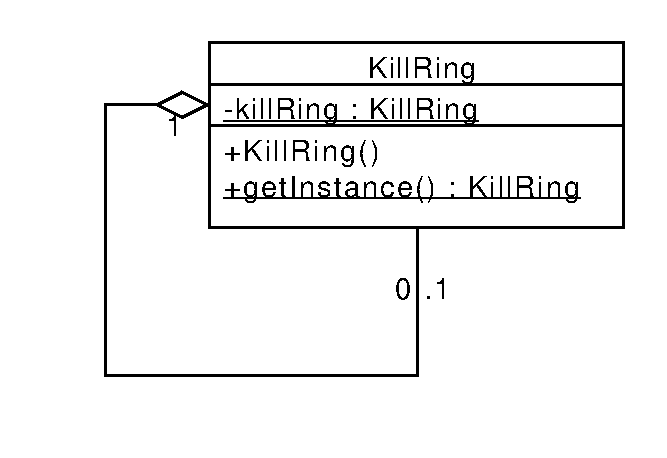
\includegraphics[width=0.5\textwidth]{singleton-killring-class-diagram.pdf}}
  \caption{KillRing class diagram}
\end{figure}
\end{center}
\subsubsection{Concrete situation description}
In this situation, the singleton pattern is used to keep track of deleted text in a single place in the application.\\
The constructor is here public. However, the common usage of the singleton pattern uses a private constructor in order to only have one instance of this class living in the system. The constructor is here made public because the plugins may want to create their own KillRing. 


\subsection{Abstract Factory}%org.gjt.sp.jedit.syntax.ModeProvider, org.gjt.sp.jedit.io.VFSManager, org.gjt.sp.jedit.gui.statusbar.StatusWidgetFactory (abstract factory) avec BufferSetWidgetFactory (concrete factory) avec Widget (abstract product) avec org.gjt.sp.jedit.gui.StatusBar (client)
The org.gjt.sp.jedit.gui.statusbar.StatusWidgetFactory is an example of the abstract factory pattern.

\subsubsection{Purpose}
Creational pattern.
\subsubsection{Participants}
The participants are the classes : org.gjt.sp.jedit.gui.statusbar.StatusWidgetFactory, org.gjt.sp.jedit.gui.statusbar.BufferSetWidgetFactory, org.gjt.sp.jedit.gui.statusbar.BufferSetWidget, org.gjt.sp.jedit.gui.statusbar.Widget and org.gjt.sp.jedit.gui.StatusBar.

\begin{itemize}
 \item \textbf{StatusWidgetFactory} : Abstract Factory
 \item \textbf{BufferSetWidgetFactory} : Concrete Factory
 \item \textbf{BufferSetWidget} : Concrete Product
 \item \textbf{Widget} : Abstract Product
 \item \textbf{StatusBar} : Client
\end{itemize}

\subsubsection{Class diagram}
\begin{center}
\begin{figure}[h]
  \centerline{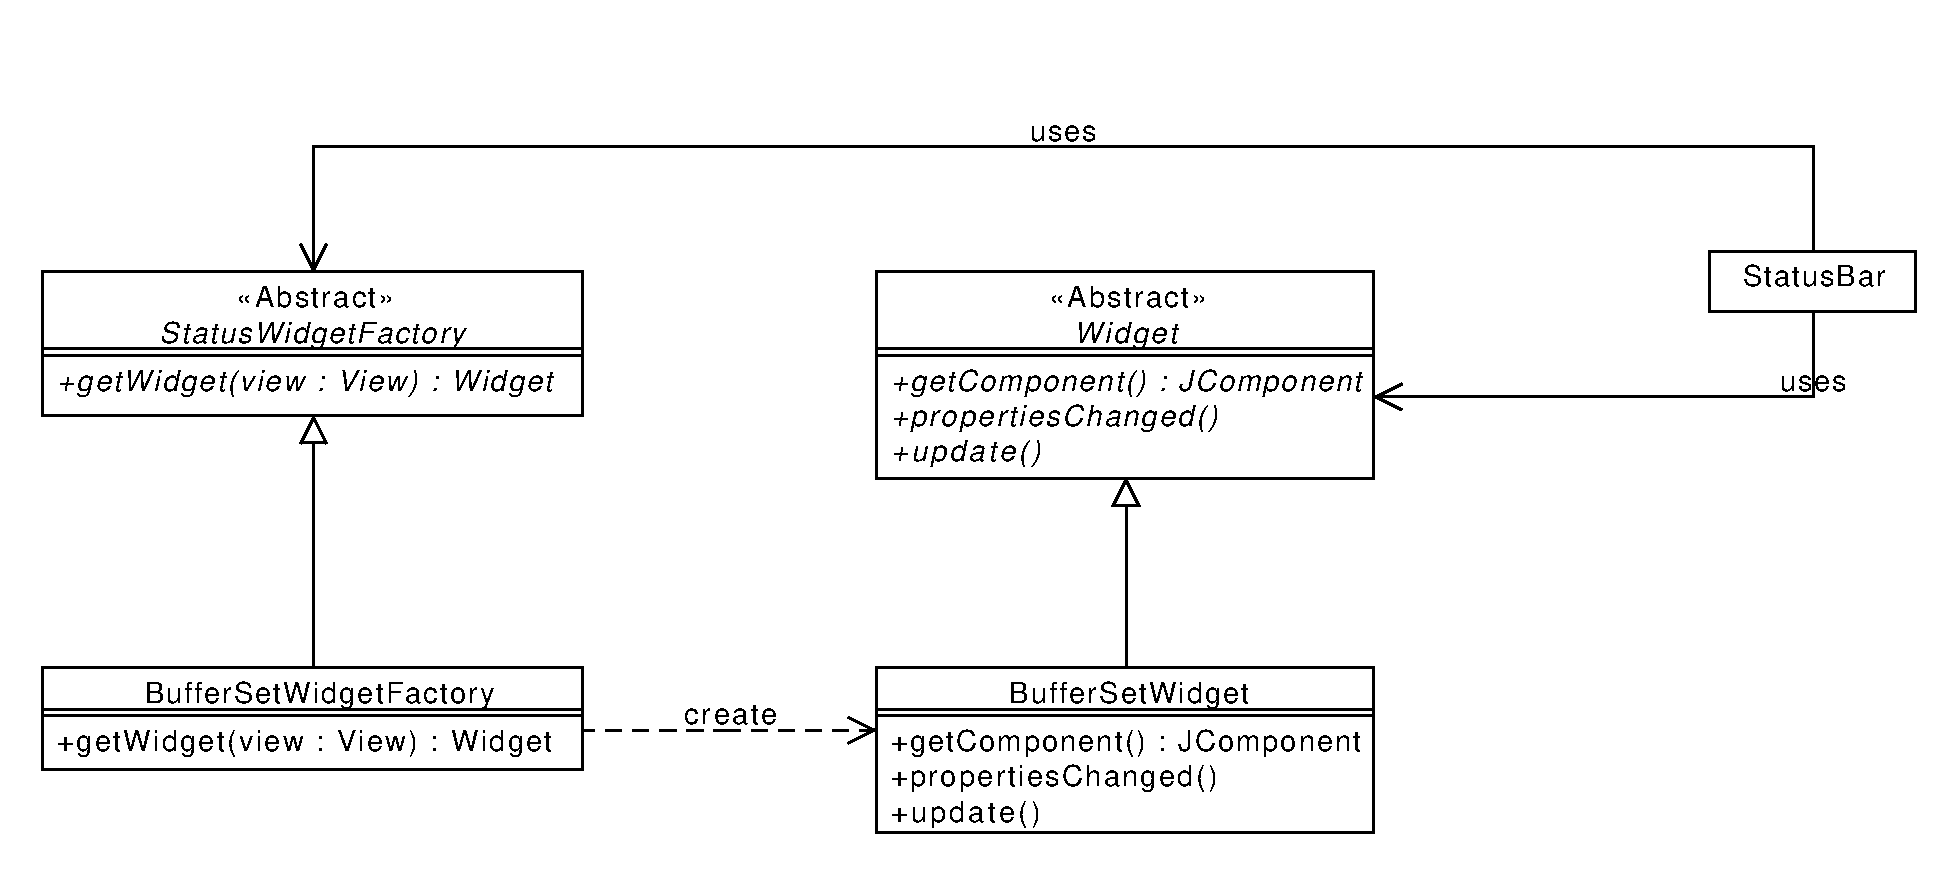
\includegraphics[width=0.7\textwidth]{abstractfactory-statuswidgetfactory-class-diagram.pdf}}
  \caption{StatusWidgetFactory class diagram}
\end{figure}
\end{center}
\subsubsection{Concrete situation description}
In this situation, the abstract factory pattern is used to let a StatusBar object creating different kind of Widget without specifying their concrete class. 

\subsection{Observer}

\subsubsection{Purpose}

\subsubsection{Participants}

\subsubsection{Class diagram}

\subsubsection{Concrete situation description}


\subsection{Adapter}
The org.gjt.sp.jedit.buffer.BufferAdapter is an example of the adapter pattern.

\subsubsection{Purpose}
Structural pattern.
\subsubsection{Participants}
The participants are the classes : org.gjt.sp.jedit.buffer.BufferAdapter, org.gjt.sp.jedit.buffer.BufferListener, a client and a target.
\begin{itemize}
 \item \textbf{BufferAdapter} : Adapter
 \item \textbf{BufferListener} : Adaptee
\end{itemize}

\subsubsection{Class diagram}

\subsubsection{Concrete situation description}


\subsection{Visitor}

\subsubsection{Purpose}

\subsubsection{Participants}

\subsubsection{Class diagram}

\subsubsection{Concrete situation description}


\section{Exercise 2 : Recognize Design Patterns}
Design pattern found :
\begin{itemize}
\item Composite, structural design pattern
\item Command, behavioural design pattern
\end{itemize}
Composite participants :
\begin{itemize}
\item Component : CoumpoundEdit
\item Leaf : Edit
\item Composite : CoumpoundEdit
\end{itemize}
Command participants :
\begin{itemize}
\item Command : Edit
\item ConcreteCommand : Insert, Remove, Replace, CompressedReplace
\item Client :
\item Invoker : JEditBuffer
\item Receiver : UndoManager.buffer (JEditBuffer)
\end{itemize}
\section{Exercise 3 : Coupling and Cohesion}
\subsection{Question a}
\begin{itemize}
\item A high cohesion is preferable because it means that all the function of a class are in that class for a good reason, the class has a well defined purpose.
\item A loose coupling is better because it allow the developer to modify the content of some module without jeopardize the interaction between the module and the others.
\end{itemize}
\subsection{Question b}
\subsubsection{MiscUtilities}
The cohesion type is coincidental because this class regroup all the small functions needed at several places in the projects which therefore do not have anything in common.\\
To improve the cohesion the class could be divided in several sub classes which take care of a single feature, by example, there is several functions which focus the path, they could be regrouped in one class in order to have a logical cohesion.
\subsubsection{GUIUtilities}
This class has a logical cohesion, the class handle all the function to create the GUI, they are grouped in this class because they all act in the same purpose even though they do not interact with each other.\\
The class could be sub divided to focus on single element of the GUI per classes but it will only improve the logical cohesion, in order to achieve a functional cohesion, the functions could be dispatched where they are actually useful if possible, i.e if they are not used at several places in the project.
\subsubsection{io/VFSFile.java}
This class represent an ADT, therefore the cohesion is maximal.
\subsection{Question c}
It seems that the coupling between these two classes is of the type Data because some data shared between the modules are done through parameters (e.g advanceSplashProgress).


\end{document}
